\section{State of the Art}
In diesem Kapitel werden verwandte Arbeiten zum Thema dieser Arbeit vorgestellt. Außerdem wird erläutert, inwiefern die vorgestellten Arbeiten sich zum Lösen der gestellten Aufgabe eignen.\\
Ich unterteile meine Arbeit hierbei in die Oberpunkte \textit{Objekterkennung}, zum Detektieren der Objekte und Bestimmen der Lage, und das \textit{Schätzverfahren}, zur Bestimmung und Vorhersage des Objektverlaufs.
\subsection{Objekterkennung}
Bei der Objekterkennung unterscheide ich grob zwischen Ansätzen, die Objekte aufgrund von Linien und deren Beziehungen detektieren und solchen, die andere Objekteigenschaften nutzen.
\subsubsection{Linienerkennung}
Linienförmige Objekte heben sich unter anderem durch zwei annähernd parallel verlaufende Kanten vom Hintergrund ab.
Ein verwandtes Problem hierzu ist die Detektion eines Straßenverlaufs, der sich ebenso durch zwei fast parallele Linien (den Fahrbahnmarkierungen) auszeichnet [Abb. \ref{Abb. 4}].\\
\begin{figure}[H]
	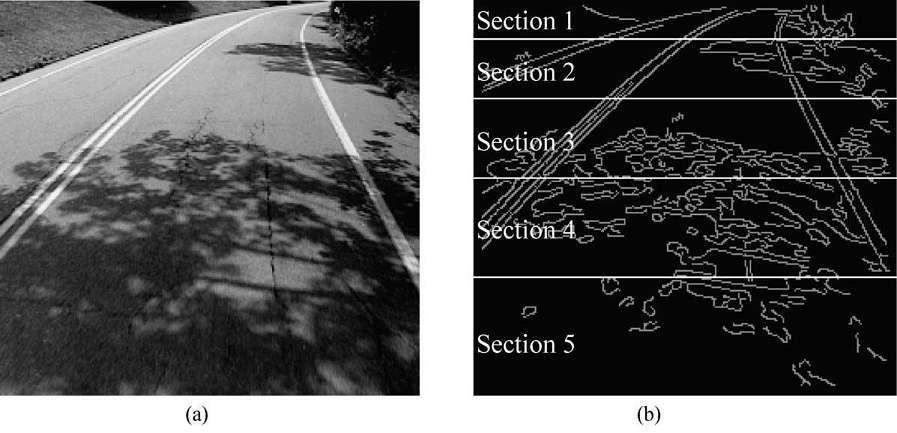
\includegraphics[scale=0.5]{SOTA/roadEdges.jpg}
	\caption[Typischer Straßenverlauf mit entpsrechendem Kantenbild]{Ein typischer Straßenverlauf mit entsprechendem Kantenbild und dem Ansatz der vertikalen Unterteilung in mehrere Segmente aus \texttt{Lane detection and tracking using B-Snake}\cite{wang2004lane}.}
	\label{Abb. 4}
\end{figure}

Viele Arbeiten zum Tracking von Fahrbahnmarkierungen basieren auf der Kantenextraktion (\cite{Voisin2005},\cite{bai2010multiple}, \cite{Park20032301},\cite{wang2004lane}). Aus dem Kantenbild werden dann die Charakteristiken der Straße extrahiert.
Hierfür wird oft versucht, mithilfe von LCFs (lane-curve-function) die Markierungen zu finden. Dies eignet sich besonders gut, um den typischen Straßenverlauf in Form von leichten Kurven zu erkennen. Eine LCF stellt ein Modell des gekrümmten Straßenverlaufs dar, das sich durch Parameter bestimmen lässt. Hierbei unterscheidet sich die LCF in zwei Breiche. Zum einen einen geraden Beginn, gefolgt von einem gekrümmten Bereich.\\
Jong Woung Park et al.\cite{Park20032301} untersuchen Straßenbilder mithilfe von LCFs und einem Krümmungsindex, der die Richtung und Stärke der Krümmung beeinflusst. Bestimmt wird dabei, ob es sich im Bild um eine gerade, nach links oder nach rechts gebogene Straße handelt.\\
Die Methode setzt dabei voraus, dass die geraden Anfänge der Straßenmarkierungen nah an der Kamera sowie der \textit{vanishing point} \todo{glossar?}bereits erkannt wurden. Der \textit{vanishing point} ist der Punkt, an dem sich parallele Linien projziert auf die Bildebene schneiden (vgl. Abb. \ref{detHough}). Aus diesem Wissen werden zunächst die von der Krümmung unabhängigen Parameter der LCF berechnet. Der Bereich weiter entfernt von der Kamera bestimmt dann die Krümmung der gesuchten LCF. Hierfür wird für die verschiedenen Krümmungen eine \textit{region of interest} (ROI) um die LCF definiert. Innerhalb der ROI wird dann mithilfe von Kantenerkennung evaluiert, welcher Krümmungsgrad am ehesten den Fahrbahnverlauf abbildet. Dieses Verfahren ist in Abbildung \ref{lcfDec} zu sehen, in dem die ROI der Linkskurve das beste Ergebnis liefert.
\begin{figure}[H]
	\centering
	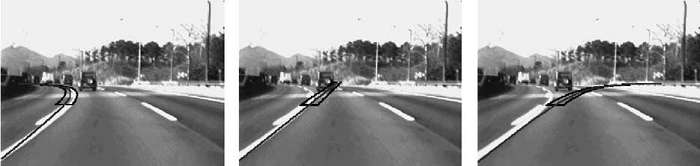
\includegraphics[width=\textwidth,height=0.2\textheight]{SOTA/lcfResult.jpg}
	\caption[Detektion eines Straßenverlaufs über eine LCF]{Detektion des Straßenverlaufs mithilfe von LCF und ROI. Die schwarz umrahmte Fläche bestimmt die ROI. Die Kurven der drei Bilder werden durch verschiedene Krümmungindizes der LCF erzeugt. Die von der Krümmung unabhängigen Parameter der LCF sind in allen Bildern gleich.}
	\label{lcfDec}
\end{figure}

Alternativ können auch gerade Linien im Kantenbild gesucht werden. In \texttt{A Real-time Lane Detection Algorithm Based on a Hyperbola-Pair Model} \cite{chen2006real} suchen Chen et al. mithilfe des \textit{\rans}-Algorithmus auf einem Kantenbild zwei gerade Linien. Auf Grundlage der gefundenen Linien wird anschließend die Mitte der Straße und in weiteren Schritten der Straßenverlauf bestimmt [Abb. \ref{ransDetectChen}].\\
\begin{figure}[H]
\centering
\begin{tabular}{cc}
\subfloat[Ursprungsbild mit Linien- und Horizontmarkierungen]{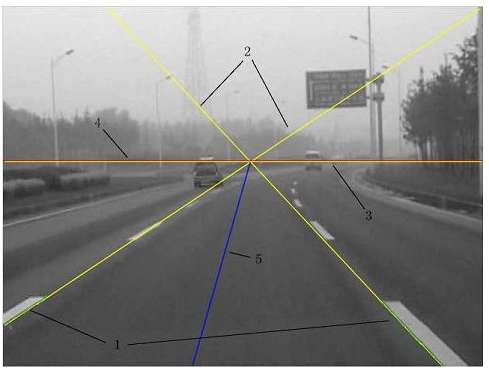
\includegraphics[width=0.5\textwidth,scale=0.5]{SOTA/orgRansDet.jpg}}&
\subfloat[Kantenbild mit Bereichen zwischen zwei Linien und Mitte der Straße]{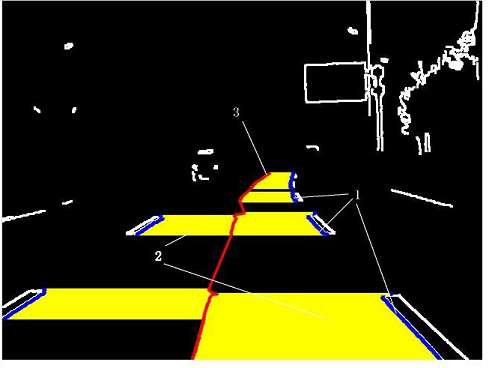
\includegraphics[width=0.5\textwidth,scale=0.5]{SOTA/edgesRansDet.jpg}}
\end{tabular}
\caption[Detektion eines Straßenverlaufs mit dem \rans -Algorithmus]{Erkennungsprozess aus \textit{A Real-time Lane Detection Algorithm Based on a Hyperbola-Pair Model}. Im rechten Bild ist in rot die detektierte Straßenmitte gekennzeichnet.}
\label{ransDetectChen}
\end{figure}
Einen ähnlichen Ansatz verfolgen auch Wang et al. für ihre Detektion in \texttt{Lane detection and tracking using B-Snake}\cite{wang2004lane}. Besonders hierbei ist, dass das Eingabebild vertikal in fünf Segmente eingeteilt wird (siehe Ab. \ref{Abb. 4}). In jedem Segment werden mithilfe der \textit{Hough Transformation} Linien erkannt und wie bei Chen die Mitte der Straße bestimmt. Außerdem wird für jedes Segment auch der \textit{vanishing point} bestimmt. Der \textit{vanishing point} eines Segmentes bestimmt die Richtung der detektierten Straße (siehe Abb. \ref{detHough}).\\
Die Arbeit bietet eine Möglichkeit innerhalb eines Bildes eine Kurve zu detektieren, obwohl nur gerade Linien gesucht wurden.
\begin{figure}[H]
\centering
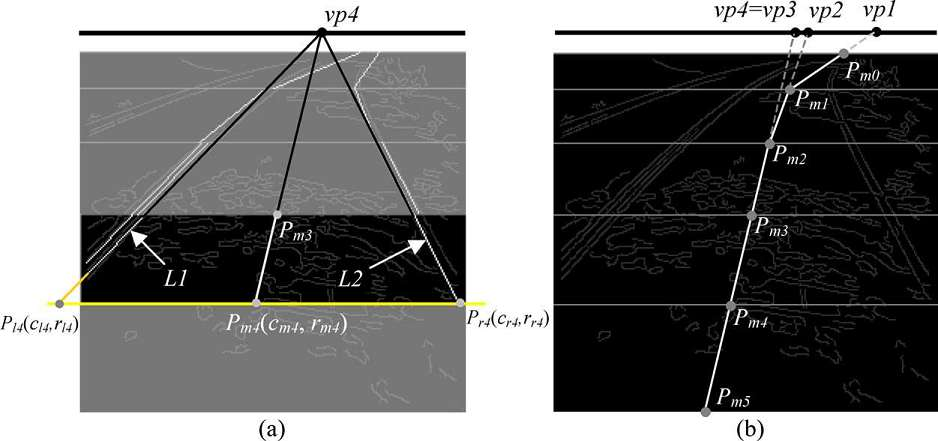
\includegraphics[scale=0.5]{SOTA/edgesSection.jpg}
\caption[Detektion eines Straßenverlaufs mit der \textit{Hough Transformation}]{Ergebnis der Straßenverlaufsdetektion mithilfe von \textit{Hough Transformation} nach Wang et al.. Links werden die erkannten Straßenmarkierungen der Segmente angedeutet und der \textit{vanishing point (vp)} des vierten Segmentes. Rechts ist die final detektierte Mittellinie der Straße über alle Segmente.}
\label{detHough}
\end{figure}
Aus den von mir betrachteten Arbeiten geht hervor, dass mithilfe von LCFs kurvige Straßenverläufe gut erkannt werden können. Da Kameras in den betrachteten Arbeiten jedoch nach vorne ausgerichtet sind, um den Straßenverlauf möglichst weit zu erkennen, unterscheidet sich dieser Ansatz in einem wesentlichen Punkt vom Unterwasserszenario. In den meisten Einsatzgebieten würde eine nach vorn ausgerichtete Kamera keine Objekte am Meeresboden sehen können. Der Höhenunterschied von der Kamera zum Boden wäre zu groß um Objekte nah am Fahrzeug zu sehen und in der Entfernung sind oftmals, bedingt durch schlechte Sichtverhältnisse, keine Objekte erkennbar. Aus diesen Gründen sollte die Kamera gerade nach unten oder leicht nach vorne geneigt ausgerichtet sein.\\
Aus dieser Ausrichtung resultiert jedoch, dass der betrachtete Bereich weitaus kleiner ist und die meisten Objekte nur eine sehr leichte Krümmung im Bild aufweisen. In solch kleinen Bereichen reicht eine Linienerkennung aus.

\subsubsection{Andere Ansätze}
Im \texttt{CSurvey}-Projekt \cite{Albiez2015CSurveyA} beleuchten Albiez et al. eine Pipeline mit einem Linienlaser und erkennen die Linie im Kamerabild über den Helligkeitswert. Für die Detektion wird für jede Bildzeile ein Helligkeitsmaximum gesucht. Hierfür wird ein Template, das den typischen Helligkeitsunterschied der beleuchteten Pipeline zum Hintergrund abbildet, auf die Zeile angewandt [Abb. \ref{templateCSurv}].\\
Diese Detektion wurde vor allem in verschiedenen Entfernungen zum Boden und verschiedenen Trübheitsgraden des Wassers getestet. Ein Ergebnis der Arbeit ist, dass mit dem Template auch bei schlechter Sicht die Pipeline noch erkennbar ist. Jedoch wird ab einem bestimmten Trübheitsgrad das gesamte Bild zu hell für eine Erkennung, da die Reflexion des Laserlichts im trüben Wasser viel zu groß ist.\\
\begin{figure}[H]
\centering
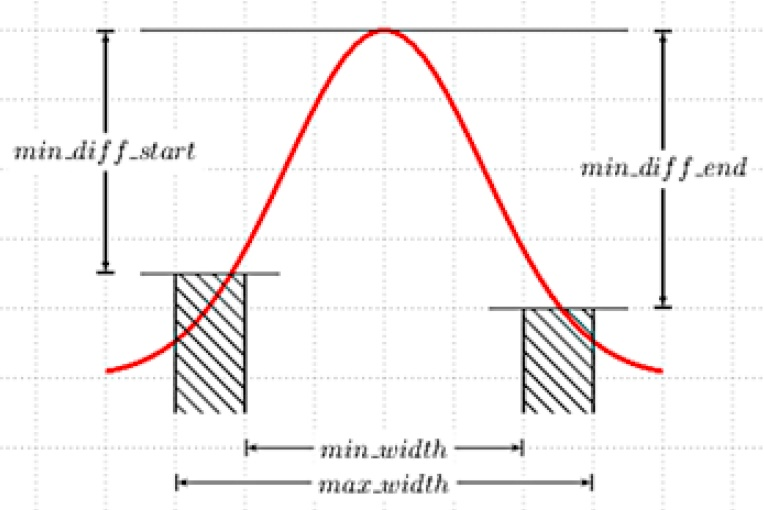
\includegraphics[scale=0.6]{SOTA/templateCSurvey.jpg}
\caption[Template zur Pipelinedetektion aus \textit{CSurvey}]{Template zur Detektion auf Helligkeitsdaten aus \textit{CSurvey}.}
\label{templateCSurv}
\end{figure}
Im \texttt{Avalon}-Projekt \cite{avalon} wird eine Pipeline mit einem Farbfilter im HSV-Farbraum detektiert. Dieser Filter erzeugt zuerst ein Binärbild. Auf diesem Binärbild wird dann mit einem Canny Edge Detector ein Kantenbild generiert. Im Kantenbild wird mithilfe der Hough-Transformation nach Linien gesucht.\\
In \texttt{Simple vision tracking of pipelines for an autonomous underwater vehicle}\cite{hallset1991simple} wird ähnlich wie bei den Linienerkennungsansätzen eine Kantenerkennung durchgeführt. Im Kantenbild werden dann durch Segmentierung Regionen definiert, auf welche dann umschließende Rechtecke gelegt werden.
Aus diesen Rechtecken lässt sich dann die gesuchte Pipeline bestimmen.\\
\begin{figure}[H]
\centering
\begin{tabular}{cc}
\subfloat[Originalbild nach Kontrastverstärkung]{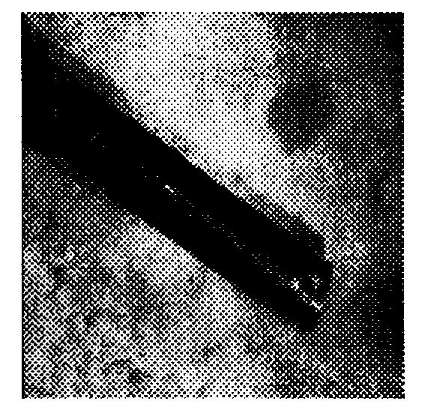
\includegraphics[scale=0.4]{SOTA/rectangleFirst.jpg}}&
\subfloat[Kantenbild durch Sobel-Filter]{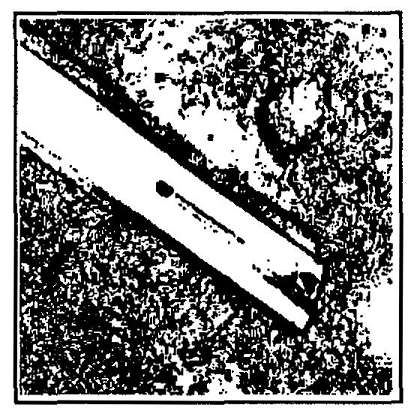
\includegraphics[scale=0.4]{SOTA/rectangleSec.jpg}}\\
\subfloat[Segmentiertes Bild]{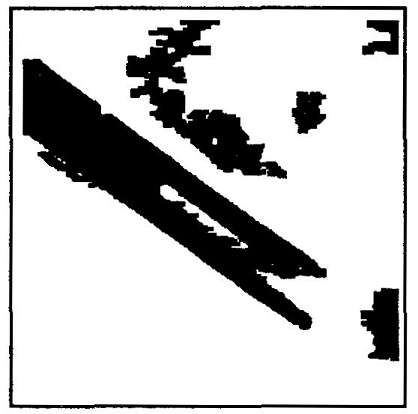
\includegraphics[scale=0.4]{SOTA/rectangleThir.jpg}}&
\subfloat[Erkannte Rechtecke]{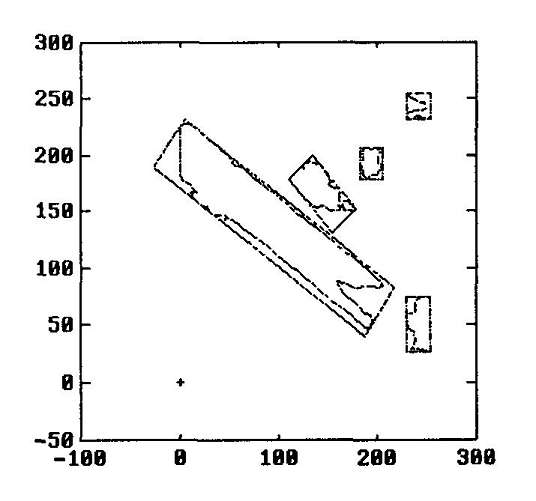
\includegraphics[scale=0.4]{SOTA/rectangleFor.jpg}}
\end{tabular}
\caption[Detektion einer Pipeline im Kantenbild]{Einzelschritte der Erkennung aus \textit{Simple vision tracking of pipelines for an autonomous underwater vehicle}. Die Pipeline wird hierbei durch das Untersuchen des Kantenbildes auf rechteckige Strukturen detektiert.}
\label{rectDetect}
\end{figure}

Foresti et al. detektieren in \textit{A Vision Based System for Object Detection in
Underwater Images}\cite{foresti2000vision} Unterwasserpipelines mithilfe eines neuronalen Netzes. In Abbildung \ref{nnDet} ist zu sehen, dass die Pipelines sehr gut erkannt wurden. Selbst bei vom Sand verdeckten Pipelines (\ref{nnDet}c und \ref{nnDet}d) werden die Kanten der Pipelines noch richtig bestimmt.

\begin{figure}[H]
\centering
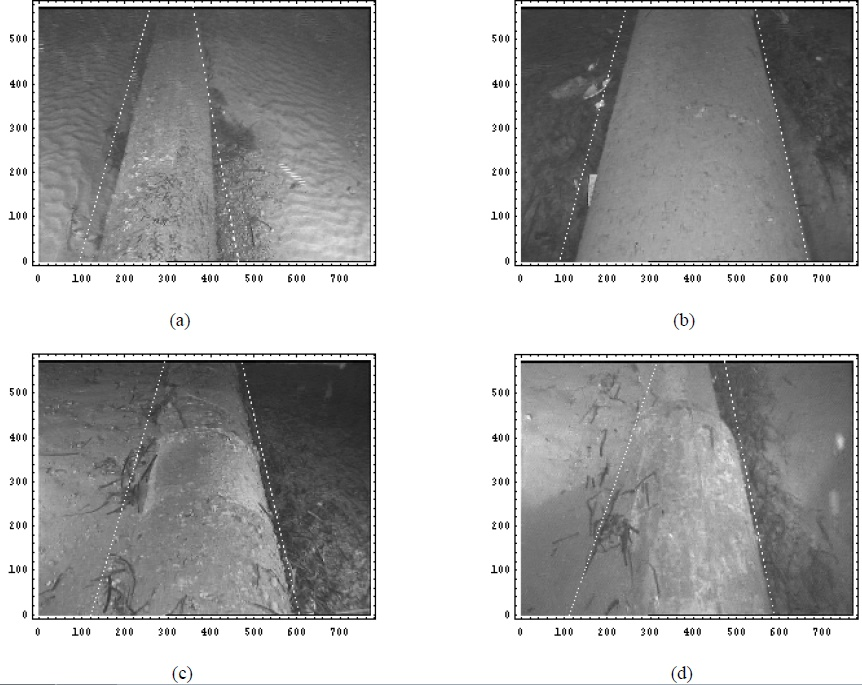
\includegraphics[width=\textwidth,height=0.3\textheight]{SOTA/nnpiperesults.jpg}
\caption[Pipelinedetektion mit neuronalem Netzwerk.]{Pipelines erkannt mithilfe eines neuronalen Netzwerks aus \textit{A Vision Based System for Object Detection in Underwater Images}\cite{foresti2000vision}. Es werden selbst verdeckte Pipelines sehr gut erkannt.}
\label{nnDet}
\end{figure}
Trotz dieser guten Ergebnisse habe ich mich gegen ein neuronales Netz entschieden. Zum einen gab es zu Beginn der Arbeit keine geeigneten Trainingsbilder aus der Simulationsumgebung, um das Netz zu trainieren. Außerdem ist ein neuronales Netz stets als \textit{black box} zu betrachten und die Detektion ist nicht eindeutig nachvollziehbar. Neben diesen Faktoren ist auch der Berechnungsaufwand für ein neuronales Netz höher einzuschätzen, als bei anderen Ansätzen.\\
Aus diesen Gründen habe ich mich für einen leichter zu implementierenden, klassischeren Ansatz der Bildverarbeitung entschieden.

Die auf Linienerkennung basierenden Ansätze eignen sich sehr gut, solange klare Kanten im Bild erkennbar sind. Im Unterwasserszenario setzt dies gute Sicht- und Lichtverhältnisse voraus. Außerdem würden vom Meeresboden verdeckte Objekte keine oder sehr kurvige Kanten ergeben, in denen die vorgestellten Ansätze keine Ergebnisse liefern würde. Beide Voraussetzungen sind im Unterwasserbereich nicht erfüllbar, weswegen in dieser Arbeit ein anderer Ansatz gewählt wurde.\\
Sehr gut eignet sich ein helligkeitsbasierter Ansatz. Wie im \textit{CSurvey}-Projekt\cite{Albiez2015CSurveyA} gezeigt, kann ein solcher Ansatz selbst unter schlechten Sichtbedingungen noch gute Ergebnisse liefern. Es ist zu erwarten, dass auch in der verwendeten Simulationsumgebung gute Resultate erzielt werden können.\\
\subsection{Schätzverfahren}
Wie in der Einleitung beschrieben muss ein Schätzverfahren entwickelt werden, um dem Objektverlauf optimal folgen zu können. Das Verfahren muss auf der Ausgabe der Objekterkennung aufsetzen.
\subsubsection{Kalman-Filter}
Ein Kalman-Filter ist ein Ansatz, um verrauschte Messwerte zu verbessern und auch ausbleibende Messungen auszugleichen. Der Kalman-Filter basiert auf einem linearen State wie zum Beispiel der Pose und Posenänderung eines Roboters. In jedem Zeitschritt des Filters wird aufgrund des vorherigen Zustands und dem Weltmodell ein Folgezustand berechnet und dieser dann mit den aktuellen Messwerten verglichen.(vgl. \textit{Optimal State Estimation, Chapter 5}\cite{simon2006optimal}).
In \textit{Real-Time Visual Tracking of a Moving Object Using Pan and Tilt Platform: A Kalman Filter Approach}\cite{torkaman2012real} nutzen Bahare Torkaman und Mohammad Farrokhi einen Kalman-Filter, um die Bewegung eines Objektes, das mit einer Kamera detektiert wird, zu verfolgen (siehe Abb. \ref{kalmanFilter}). Der State des Kalman-Filters ist dabei die \textit{x}- und \textit{y}-Position des Objektes in der Ebene, sowie dessen aktuelle Positionsänderung. Der Zustandsübergang wird durch die Objektbewegung durchgeführt. Das Update der Messung besteht aus der erkannten Position der Objekterkennung.\\
In der Arbeit ist sehr gut zu sehen, wie der Kalman-Filter den Fehler der Objekterkennung nahezu halbiert.\\
\begin{figure}[H]
\centering
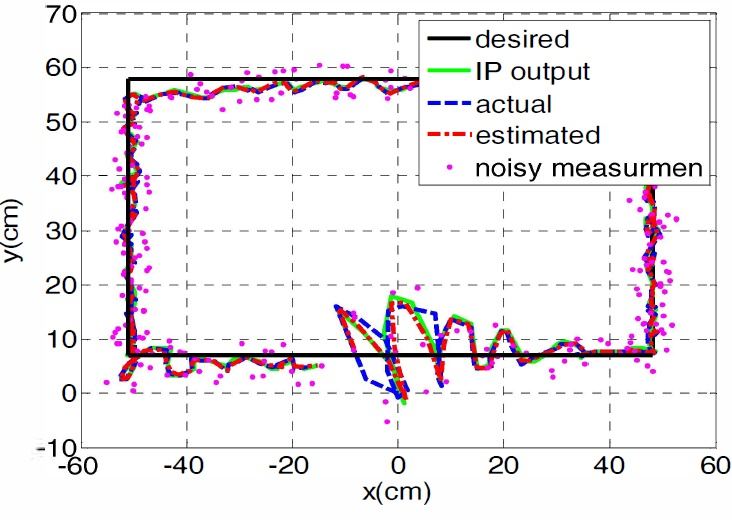
\includegraphics[scale=0.8]{SOTA/Kalman.jpg}
\caption[Schätzung einer Objektbewegung mit Kalman-Filter.]{Eine Objektbewegung wird mit einem Kalman-Filter verfolgt. Lila sind hierbei die Positionsbestimmungen aus der Bilderkennung, blau der wirkliche Objektverlauf, grün der vom Zustandsübergang des Kalman-Filters erwartete Verlauf und rot der vom Kalman-Filter korrigierte Verlauf.}
\label{kalmanFilter}
\end{figure}
\todo{nochmal checken was hier was ist}
Der Kalman-Filter eignet sich jedoch nicht gut für das gestellte Szenario. Um den Messfehler der Objekterkennung auszugleichen, müsste der State des Kalman-Filters das zu verfolgende Objekt abbilden. Dieser State sowie der benötigte Statewechsel sind jedoch nicht problemlos zu definieren.\\
Das Problem beim Definieren des States liegt darin, dass das Objekt selbst keine wechselnden Zustände hat, sondern stets fest bleibt. Ein Ansatz wäre, die Position und Ausrichtung des Objektes im State abzubilden. Bei einem Zustandsübergang müsste dann eine neue Position und Ausrichtung berechnet werden. Da sich das Objekt selbst nicht bewegt, müsste dieser Übergang in Abhängigkeit der Bewegung des AUVs umgesetzt werden. Es gibt jedoch keinen direkten Zusammenhang zwischen der Objektlage und der AUV Bewegung und somit kann kein Folgezustand berechnet werden. Da das Objekt keine Eigenbewegung durchführt ist die Lage stets unabhängig vom AUV. Eine von dem AUV abhängige Position wäre die nächste Position vom AUV auf dem Objektverlauf. Hierfür müsste jedoch aus den vorhandenen Daten zuerst der Objektverlauf berechnet werden, was direkt zum nächsten vorgestellten Ansatz führt.
\subsubsection{Regressionsverfahren}
Ein weiterer Lösungsansatz für das Schätzverfahren ist die Regression. Bei der Regression wird versucht, ein parametrisierbares Modell an gegebene Daten anzupassen. Dabei wird versucht, den Fehler der Daten im Bezug zur aus dem Model generierten Kurve zu minimieren.
Brundson nutzt in \texttt{Path estimation from GPS tracks}\cite{brunsdon2007path} einen Regressionsansatz, um aus fehlerbehafteten GPS-Daten einen Pfad durch ein Stadtgebiet genauer zu bestimmen. Die GPS-Daten ähneln den zu erwartenden Daten der Objekterkennung. Auch hier gibt es einen reellen Verlauf und fehlerbehaftete Messdaten zu beiden Seiten dieses Verlaufs.\\
Brundson berechnet die optimalen Modellparameter durch das Minimieren des quadrierten Fehlers jedes Punktes zur Kurve.\\
In der Abbildung \ref{gpsfit} ist gut zu sehen, wie die Kurve nahezu den echten Pfad abbildet.
\begin{figure}[H]
\centering
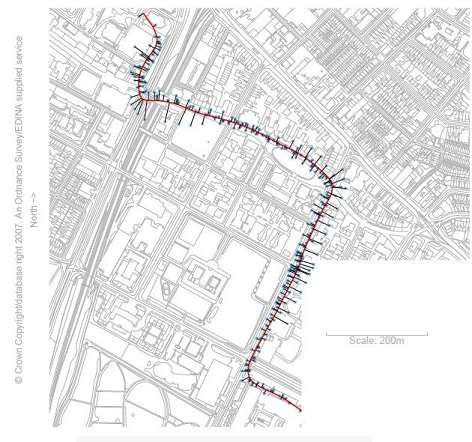
\includegraphics[scale=0.5]{SOTA/gpsCurve.jpg}
\caption[Abbildung eines Pfadverlaufs auf Basis von GPS-Daten.]{Regression angewandt auf Positionsangaben eines GPS-Empfängers aus \texttt{Path estimation from GPS tracks}\cite{brunsdon2007path}. Die Fehler zu beiden Seiten des realen Fehlers werden gut durch die berechnete Kurve ausgeglichen}
\label{gpsfit}
\end{figure}
Eine sehr ähnliche Arbeit findet sich in \texttt{Autonomous Searching and Tracking of a River using an UAV}\cite{rathinam2007autonomous} von Rathinam et al.. Ziel der Arbeit ist es mithilfe eines UAVs (Unmanned Aerial Vehicle) den Verlauf eines Flusses zu bestimmen. Das Flugzeug ist mit einer Kamera zur Detektion des Flusses ausgestattet.\\
Aus der Objekterkennung werden GPS-Positionen des Flusses berechnet. Durch diese Daten wird dann durch Regression eine Kurve gelegt (siehe Abb. \ref{riverCurve}).\\
Im gelb gekennzeichneten Bereich des rechten Bildes ist zu sehen, dass die Kurve an dieser Stelle nicht den Flussverlauf abbildet. Im selben Bereich ist im linken Bild zu sehen, dass die Objekterkennung keine Ergebnisse lieferte. Dies liegt daran, dass das Flugzeug dem engen Flussverlauf aufgrund der Trägheit der Steuerung nicht folgen konnte. Diese Trägheit ist in ähnlichen Rahmen auch im Unterwasserszenario zu erwarten.\\
Bemerkenswert ist, dass im roten Bereich ebenfalls keine Ergebnisse der Objekterkennung vorhanden sind, die Kurve jedoch trotzdem genau dem Flussverlauf folgt. Dies lässt sich darauf zurückführen, dass die letzten GPS Daten vor der Lücke die Abzweigung der Kurve andeuten, was im gelben Bereich nicht der Fall ist.
\begin{figure}[H]
\centering
\begin{tabular}{cc}
\subfloat[Flusspositionen nach Objekterkennung]{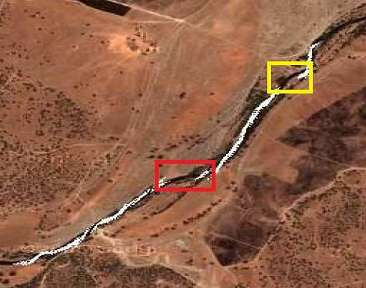
\includegraphics[scale=0.6]{SOTA/rivergps.jpg}}&
\subfloat[Flussverlauf nach Curve Fitting]{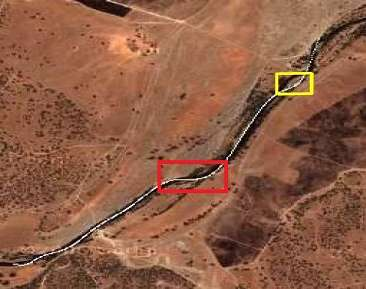
\includegraphics[scale=0.6]{SOTA/rivercurve.jpg}}\\
\end{tabular}
\caption[Abbildung eines Flusses mit Regression]{Regression angewendet auf GPS-Daten eines Flussverlaufs aus \texttt{Autonomous Searching and Tracking of a River using an UAV}\cite{rathinam2007autonomous}. Im gelben Bereich wird ein fehlender Sichtkontakt zum Fluss nicht optimal abgedeckt. Im roten Bereich ist die Kurve trotz fehlender Detektion nahezu optimal abgebildet.}
\label{riverCurve}
\end{figure}
Das Curve Fitting Verfahren eignet sich gut für die Problemstellung der Arbeit. Die zwei vorgestellten Arbeiten zeigen, dass sowohl Fehler durch Ausreißer abgefangen werden, als auch Bereiche ohne Ergebnisse der Objekterkennung gut überbrückt werden können. Die genaue Beschreibung der eingesetzten Lösung und des von mir eingesetzten Modells folgt im nächsten Kapitel.